\documentclass[journal, twoside]{IEEEtran}
\IEEEoverridecommandlockouts
% The preceding line is only needed to identify funding in the first footnote. If that is unneeded, please comment it out.
\usepackage{cite}
\usepackage{amsmath,amssymb,amsfonts}
\usepackage{algorithmic}
\usepackage{graphicx}
\usepackage{textcomp}
\usepackage{xcolor}
\usepackage{stfloats}
\usepackage{multirow}
\usepackage{listings}
\usepackage{lipsum}
\usepackage{import}
% listing settings
\lstset{
  frame = lines,
  language = C,
  basicstyle = \ttfamily\footnotesize,
  breaklines = true,
}
% listing caption redefinition
\makeatletter
\def\lst@makecaption{%
  \def\@captype{table}%
  \@makecaption
}
\makeatother

\def\BibTeX{{\rm B\kern-.05em{\sc i\kern-.025em b}\kern-.08em
    T\kern-.1667em\lower.7ex\hbox{E}\kern-.125emX}}

\begin{document}

\bstctlcite{IEEEexample:BSTcontrol} % remove dashed repeated authors

\title{Investigating Performance Improvements\\in Discrete Space Hartree-Fock Calculations\\through Graphics Processing Units\\{\large EECE542 Final Project Report}}
\author{\IEEEauthorblockN{Michel Kakulphimp}
\IEEEauthorblockA{\textit{Dept. of Electrical and Computer Engineering}\\
\textit{University of British Columbia}\\
Vancouver, Canada\\
michel@kakulphimp.net}
}

\markboth{UBC Winter 2021 EECE542: Nanoscale Modelling and Simulations}%
{}
\maketitle

\section{Introduction}

\lipsum[1]

\section{Background and Related Work}

\lipsum[1]

\subsection{Hartree-Fock Method}

\cite{szabo-ostlund}
\lipsum[1]

\begin{figure*}[h]
\centering
\includegraphics[width=7in]{figures/one-core-results.pdf}
\caption{Performance Results Per Iteration (1 CPU Thread)}
\label{perf-results-per-iteration-one-core}
\end{figure*}

\begin{figure*}[h]
\centering
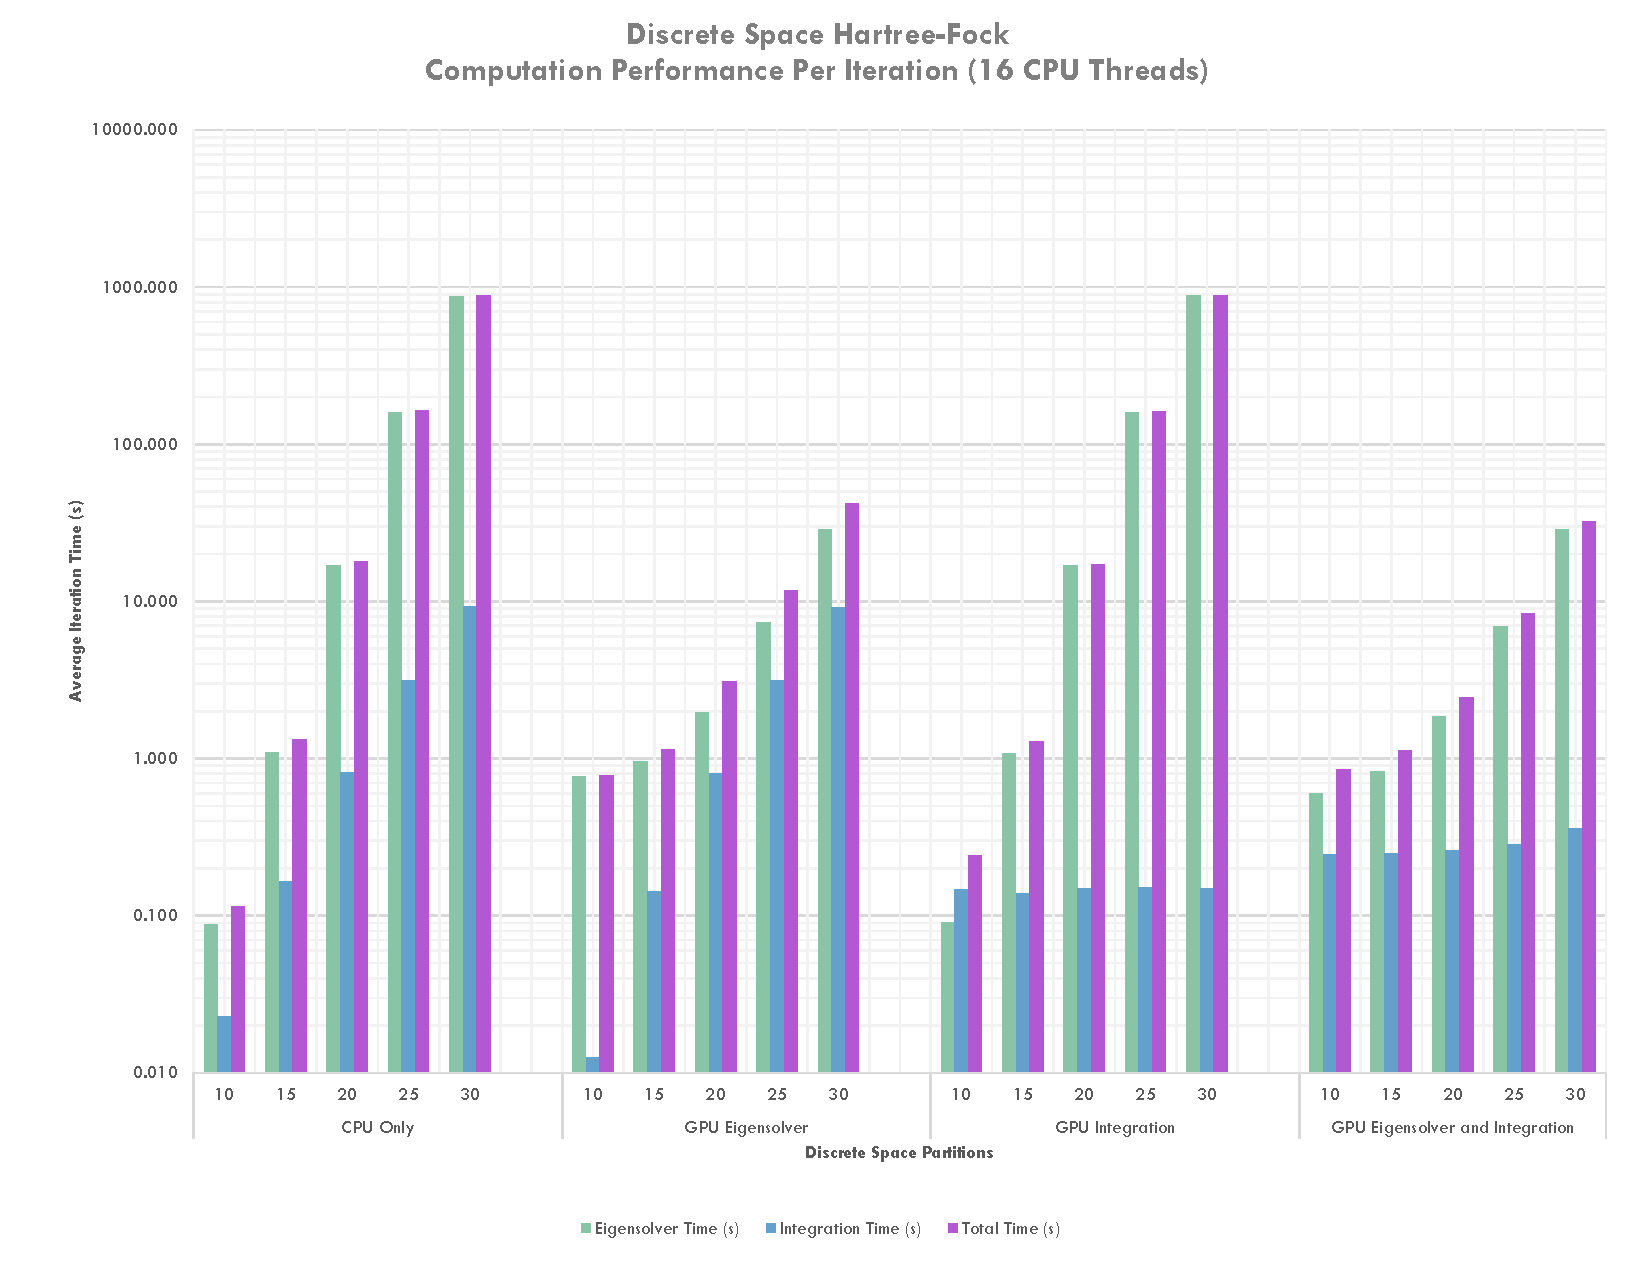
\includegraphics[width=7in]{figures/sixteen-core-results.pdf}
\caption{Performance Results Per Iteration (16 CPU Threads)}
\label{perf-results-per-iteration-sixteen-core}
\end{figure*}

\subsection{CUDA Parallel Computing Platform}

\cite{nvidia-cuda}
\lipsum[4]

\section{Acceleration Vectors}

\lipsum[4]

\subsection{Numerical Integration}

\lipsum[4]

\subsection{Eigensolver}

\lipsum[4]

\section{Implementation}

\lipsum[2]

\section{Results}

\lipsum[4]

\begin{table*}
    \renewcommand{\arraystretch}{1.3} % vertically stretch table out
    \caption{5 MB Workload Execution Times (1 millisecond dead-time)}
    \label{main-workload-results-1ms}
    \centering
    \begin{tabular}{c||c|c|c|c|c|c|c|c}
        \hline
        \multirow{2}{*}{Scaling Policy} & \multicolumn{8}{c}{Power-Loss Profile Period Sweep (Sawtooth-Down) Runtimes (s)} \\\cline{2-9}
        {} & {10 ms to 8 ms} & {S.F.} & {10 ms to 4 ms} & {S.F.} & {10 ms to 2 ms} & {S.F.} & {10 ms to 1 ms} & {S.F.} \\
        \hline
        \hline
        {Baseline}                  & {48.429} & {1.00} & {48.429}  & {1.00} & {48.429}  & {1.00} & {48.429}  & {1.00}\\
        {Linear Scaling}            & {86.326} & {1.78} & {85.405}  & {1.76} & {153.755} & {3.18} & {462.042} & {9.54}\\
        {Random Adaptive Scaling}   & {95.498} & {1.97} & {117.985} & {2.44} & {119.484} & {2.47} & {132.488} & {2.74}\\
        {Linear Adaptive Scaling}   & {95.611} & {1.97} & {94.244}  & {1.95} & {110.304} & {2.28} & {124.021} & {2.56}\\
        \hline
    \end{tabular}
\end{table*}

\begin{table*}
    \renewcommand{\arraystretch}{1.3} % vertically stretch table out
    \caption{5 MB Workload Execution Times (500 microsecond dead-time)}
    \label{main-workload-results-500us}
    \centering
    \begin{tabular}{c||c|c|c|c|c|c|c|c}
        \hline
        \multirow{2}{*}{Scaling Policy} & \multicolumn{8}{c}{Power-Loss Profile Period Sweep (Sawtooth-Down) Runtimes (s)} \\\cline{2-9}
        {} & {10 ms to 8 ms} & {S.F.} & {10 ms to 4 ms} & {S.F.} & {10 ms to 2 ms} & {S.F.} & {10 ms to 1 ms} & {S.F.} \\
        \hline
        \hline
        {Baseline}                  & {45.811} & {1.00} & {45.811}  & {1.00} & {45.811} & {1.00}  & {45.811}  & {1.00}\\
        {Linear Scaling}            & {71.445} & {1.56} & {69.302}  & {1.51} & {80.453} & {1.76}  & {255.806} & {5.58}\\
        {Random Adaptive Scaling}   & {75.260} & {1.64} & {79.272}  & {1.73} & {86.970} & {1.90}  & {95.449}  & {2.08}\\
        {Linear Adaptive Scaling}   & {65.013} & {1.42} & {74.533}  & {1.63} & {82.870} & {1.81}  & {87.939}  & {1.92}\\
        \hline
    \end{tabular}
\end{table*}

\begin{table*}
    \renewcommand{\arraystretch}{1.3} % vertically stretch table out
    \caption{Workload Execution Times (1000 microsecond dead-time)}
    \label{workload-size-performance}
    \centering
    \begin{tabular}{c||c|c|c|c|c}
        \hline
        \multirow{2}{*}{Scaling Policy} & \multicolumn{4}{c|}{Workload Runtimes (s)}\\\cline{2-6}
        {} & {5 MB} & {4 MB} & {2 MB} & {1 MB} & {R\textsuperscript{2}}\\
        \hline
        \hline
        {Baseline}                  &  {48.429} &  {38.749} &  {19.373} &   {9.688} & {1.0}\\
        {Linear Scaling}            & {462.042} & {359.176} & {154.856} &  {52.047} & {1.0}\\
        {Linear Adaptive Scaling}   & {124.021} &  {97.080} &  {47.392} &  {23.261} & {1.0}\\
        \hline
    \end{tabular}
\end{table*}

\begin{table*}
    \renewcommand{\arraystretch}{1.3} % vertically stretch table out
    \caption{5 MB Workload Execution Times (1 millisecond dead-time)}
    \label{power-loss-profile-performance}
    \centering
    \begin{tabular}{c||c|c|c|c}
        \hline
        \multirow{2}{*}{Scaling Policy} & \multicolumn{4}{c}{Power-Loss Profile (10 ms to 1 ms Sweep) Runtimes (s)} \\\cline{2-5}
        {} & {Sawtooth-Down} & {Sawtooth-Up} & {Sine} & {Square}\\
        \hline
        \hline
        {Baseline}                  &  {48.429} &  {48.429} &  {48.429} &  {48.429}\\
        {Linear Scaling}            & {462.042} & {512.373} & {523.763} & {885.978}\\
        {Linear Adaptive Scaling}   & {124.021} & {123.280} & {123.580} & {173.061}\\
        \hline
    \end{tabular}
\end{table*}

\section{Future Work}

\lipsum[4]

\section{Conclusion}

\lipsum[2]

\bibliographystyle{IEEEtran}
\bibliography{IEEEabrv, refs}

\end{document}